\documentclass[11pt,aps,preprint,nofootinbib,superscriptaddress,tightenlines]{revtex4-2}
\usepackage{amsmath,amssymb,bm,mathtools}
\usepackage{graphicx}
\usepackage{xcolor}
\usepackage{tikz}
\usepackage{algpseudocode}
\definecolor{darkblue}{RGB}{0,0,160}
\usepackage{xr-hyper}
\usepackage[colorlinks=true,linkcolor=darkblue,citecolor=darkblue,urlcolor=darkblue]{hyperref}

\def\st{\begin{equation}}
\def\stp{\end{equation}}
\def\bbeta{{\sf b}}
\def\Teff{{\sf T}}
\def\Eq#1{eq.~(\ref{#1})}
\def\Sect#1{Sect.~\ref{#1}}
\def\Fig#1{Fig.~\ref{#1}}
\providecommand{\tr}{\operatorname{tr}}
\newcommand{\avg}[1]{\langle #1\rangle}
\usepackage{dsfont}
\newcommand{\one}{\mathds{1}}
\newcommand{\tf}{\bm{\mathsf t}}

\externaldocument[PM-]{particle_metrics}
\newcommand{\EqPM}[1]{eq.~(\ref{PM-#1}) of Ref.~\cite{ParticleMetrics}}
\let\oldparagraph\paragraph
\renewcommand{\paragraph}{\par\bigskip\oldparagraph}
\begin{document}

\title{One-level (bond) dissipation on particles:\\ one and two dimensions, at rest and in motion}
\author{D.~Teaney}
\affiliation{Department of Physics and Astronomy, Stony Brook University,
Stony Brook, New York 11794, USA}
\date{\today}

\begin{abstract}
We construct a particle discretization of the viscous dissipative function of
relativistic hydrodynamics that squares differences of $\bbeta=u/T$ across
neighbouring pairs (bonds), rather than squaring a smoothed gradient.  In one
dimension at rest the bond form is the quadratic form of a graph Laplacian.  It
is exact for linear profiles on any arrangement, conserves momentum bond by
bond, and, unlike the two-level form, has no null mode.  In two dimensions
the plain bond form dissipates rigid rotation and has a single viscosity.
Subtracting a mean-field rotation and dilation from each bond, with the mean
field the least-squares fit to the bond differences, fixes both.  The rotation
is variational, so the faces of each particle carry no net torque and the
rotation exerts no mean-field force; the dilation is not, and carries the bulk
viscosity.  For a moving fluid the same construction holds with three
substitutions: bonds are measured by their comoving length, contracted with the
comoving metric $\ell^{ij}=\delta^{ij}-v^iv^j$, and the scalar part is removed
along the density-frame projector $P_{ij}$.  The continuum limit is then the
full density-frame tensor $\kappa^{ijmn}(v)$.
\end{abstract}

\maketitle

\paragraph{Purpose.}  These notes explain the equations of the construction:
the bond form in 1D, its extension to 2D with mean-field rotation and
dilation, and to a moving fluid.  Numerical tests, Fourier analyses, and
comparisons with the code are not included.

%=============================================================================
\section{Setting}
\label{sec:setting}

\paragraph{Particles and smoothed fields.}
$N$ particles sit on a periodic line at positions $x_a$.  Each carries an
entropy $s_a$ and a momentum $m_a$.  The smoothed entropy and momentum
densities are
\st
S(x)=\sum_b s_b\,W(x-x_b),\qquad M(x)=\sum_b m_b\,W(x-x_b),
\stp
with the one-dimensional Wendland C2 kernel
\st
W(r)=\frac{3}{4h}\Big(1-\frac{q}{2}\Big)^4(1+2q),\qquad q=\frac{|r|}{h}<2,
\label{W}
\stp
which is normalized, $\int W\,dr=1$, and has support $|r|<2h$.

\paragraph{Particle volume.}  Each particle is assigned the volume (in 1D, the
length) that its entropy occupies at the local entropy density,
\st
V_a=\frac{s_a}{S_a},\qquad S_a\equiv S(x_a)=\sum_bs_b\,W(x_a-x_b).
\label{Va}
\stp
$V_a$ is the quadrature weight of SPH:
\st
\sum_aV_a\,f(x_a)\simeq\int dx\,f(x).
\stp
On a uniform lattice of spacing $a$ with equal $s_a$, $V_a=a$ (up to the
discrete kernel normalization $\sum_raW(r)\simeq1$).

\paragraph{Energy, velocity and temperature.}  The energy $H$ is a
function of the smoothed fields.  Its derivatives define the particle velocity
and the (effective) temperature,
\st
\dot x_a=\frac{\partial H}{\partial m_a},\qquad
T_a=\frac{\partial H}{\partial s_a},\qquad
\bbeta_a\equiv\frac{\dot x_a}{T_a}.
\stp
In the code, to linear order at rest,
\st
\dot x_a=\sum_b V_b\,v_b\,W(x_a-x_b),\qquad v_b=\frac{M_b}{w_b},
\stp
so $\bbeta_a$ is the fluid velocity smoothed \emph{twice}.

\paragraph{The dissipative step.}
Dissipation is described by a dissipative function $K[\bbeta]\ge0$, quadratic
in $\bbeta$.  The viscous update at fixed positions is
\st
\dot m_a=-\frac{\partial K}{\partial \bbeta_a},\qquad
\dot s_a=-\bbeta_a\,\dot m_a .
\label{generic}
\stp
The second equation keeps the energy fixed:
\st
\dot H=\sum_a\big(\dot x_a\,\dot m_a+T_a\,\dot s_a\big)
=\sum_a\big(\dot x_a-T_a\bbeta_a\big)\,\dot m_a=0 ,
\stp
since $T_a\bbeta_a=\dot x_a$.  The total entropy grows,
\st
\dot S_{\rm tot}=\sum_a\bbeta_a\frac{\partial K}{\partial\bbeta_a}=2K\ge0,
\stp
using that $K$ is quadratic.  Any $K$ built from differences of $\bbeta$
conserves total momentum.  Such a $K$ is unchanged by $\bbeta_a\to\bbeta_a+c$,
so
\st
\sum_a\dot m_a=-\sum_a\frac{\partial K}{\partial\bbeta_a}=0 .
\stp

\paragraph{The continuum target.}
In one dimension the strain has a single component $\partial_x\bbeta$, and
\st
K=\frac12\int dx\;T\kappa\,(\partial_x\bbeta)^2,\qquad
\kappa\equiv\kappa^{xxxx}=2\eta\,\frac{d-1}{d}+\zeta
\;\Big(=\tfrac43\eta+\zeta\text{ for } d=3\Big),
\label{Kcont}
\stp
where $d$ is the physical dimension (the simulation is one-dimensional, but
$\eta$ and $\zeta$ are those of a $d$-dimensional fluid).  At rest $T$ is
uniform and $T\bbeta=v$, so
\st
\dot M=\partial_x(\kappa\,\partial_xv) .
\stp
A longitudinal momentum wave $m\propto\cos kx$ therefore decays at
\st
\Gamma_{\rm phys}(k)=\frac{\kappa}{w}\,k^2,\qquad w=e+p .
\label{Gphys}
\stp
(In the full equations this wave is a sound wave and $\Gamma_{\rm phys}$ is
twice its amplitude damping rate; here we freeze the particles and
study only the dissipative step, so there is no oscillation.)

%=============================================================================
\section{The two-level form}
\label{sec:twolevel}

The two-level form discretizes \Eq{Kcont} literally.  The first level is
the standard SPH gradient of $\bbeta$ at each particle:
\st
\varepsilon_a=\frac{1}{S_a}\sum_b s_b\,(\bbeta_b-\bbeta_a)\,
\partial_{x_a}W(x_a-x_b) .
\label{eps}
\stp
The second level squares it with the particle volume as the quadrature weight:
\st
K_{2L}=\frac12\sum_aV_a\,T_a\kappa_a\,\varepsilon_a^2 .
\label{K2L}
\stp
Differentiating gives the force
\st
F_a=\sum_bs_as_b\,\partial_{x_a}W(x_a-x_b)\,\big[A_a+A_b\big],\qquad
A_a=\frac{T_a\kappa_a\,\varepsilon_a}{S_a^2},
\label{f2L}
\stp
which is antisymmetric in each pair, so momentum is conserved.

The force on particle $a$ depends on $\varepsilon_b$ at every neighbour $b$
within $2h$.  Each $\varepsilon_b$ in turn depends on $\bbeta_c$ within $2h$ of
$b$.  The stencil is therefore $4h$ wide (\Fig{fig:stencil}).  More
importantly, $\bbeta$ enters only through a smoothed gradient.  Any pattern of
$\bbeta$ that this gradient does not see costs nothing in $K_{2L}$ and is not
damped.

%=============================================================================
\section{The one-level (bond) form}
\label{sec:onelevel}

\paragraph{Bond weight.}
Define the bond vector and a bond weight
\st
r_{ab}=x_b-x_a,\qquad \psi_{ab}=\psi(|r_{ab}|) .
\label{psi}
\stp
The one-level form does \emph{not} require $\psi$ to be related to the kernel
$W$.  It is an independent function, subject to:
\begin{enumerate}
\item[(P1)] \emph{Symmetric and non-negative}, $\psi_{ab}=\psi_{ba}\ge0$.  This
  gives momentum conservation and entropy production bond by bond (below).
\item[(P2)] \emph{Connected}: $\psi>0$ at least for nearest neighbours.  Then the
  only zero mode of $K$ is $\bbeta=$ const, which is the one momentum
  conservation requires.
\item[(P3)] \emph{Short range}, with range $\ell_\psi$.  The range sets both the
  long-wavelength error, $O(k^2\ell_\psi^2)$, and the damping of unresolved
  modes, $\sim\kappa/(w\ell_\psi^2)$.
\item[(P4)] \emph{Continuous}, finite at $r=0$, and going to zero continuously
  (preferably with its derivative) at the cutoff.  The particles move, and a
  jump in $\psi$ would make the force jump whenever a neighbour crosses the
  cutoff.
\item[(P5)] \emph{Normalization is irrelevant}: it is divided out by $n_a$ in
  \Eq{K1L}.
\end{enumerate}
In 2D and 3D, $\psi$ must also depend only on $|r|$ (or on the comoving distance
when the fluid moves), and its second moment must be isotropic.
Ref.~\cite{ParticleMetrics} enforces this with a moment correction $\Lambda_a$.
Our default is the Brookshaw weight built from the Wendland kernel,
\st
\psi(r)=-\frac{W'(r;h_\psi)}{r}\propto\Big(1-\frac{|r|}{2h_\psi}\Big)^3,
\qquad h_\psi=h,
\label{psidefault}
\stp
the weight of the standard SPH second derivative~\cite{Brookshaw1985}.  The
range $h_\psi\le h$ is a parameter.  A shorter range damps unresolved modes more
strongly, but leaves fewer neighbours, which makes the fit noisier and, in 2D,
the moment correction of Ref.~\cite{ParticleMetrics} less stable; the default
is $h_\psi=h$.

\paragraph{The dissipative function.}
Instead of squaring a gradient, square the bond differences:
\st
\boxed{\;K_{1L}=\frac12\sum_aV_a\,T_a\kappa_a\sum_{b\neq a}w_{ab}\,
(\bbeta_b-\bbeta_a)^2,\qquad
w_{ab}=\frac{V_b\,\psi_{ab}}{n_a},\qquad
n_a=\sum_{b\neq a}V_b\,\psi_{ab}\,r_{ab}^2 .\;}
\label{K1L}
\stp
The normalization $n_a$ is fixed by the continuum limit: the normalized bond
weights satisfy
\st
\sum_{b\neq a}w_{ab}\,r_{ab}^2=1 .
\stp
For a linear
profile the bond differences are exact,
\st
\bbeta_b-\bbeta_a=\partial_x\bbeta\;r_{ab},
\stp
and the inner sum is $(\partial_x\bbeta)^2$.  Hence
\st
K_{1L}=\frac12\sum_aV_a\,T_a\kappa_a\,(\partial_x\bbeta)^2
\;\longrightarrow\;\frac12\int dx\,T\kappa\,(\partial_x\bbeta)^2 .
\stp
This holds on \emph{any} particle arrangement, not just a lattice, because
$n_a$ is defined by the same sum.  For smooth non-linear profiles the next
correction to the squared bond difference is odd in $r$, and cancels on a
symmetric neighbourhood.  The weights belong to particle $a$, so $w_{ab}\neq
w_{ba}$ in general.  $K_{1L}$ is the quadratic form of a graph Laplacian on the
bonds, normalized so that for any smooth field $\phi$
\st
\sum_{b\neq a}w_{ab}(\phi_b-\phi_a)\simeq\frac12\,\partial_x^2\phi .
\stp
Ref.~\cite{ParticleMetrics}, Sec.~\ref{PM-sec:weights}, collects the general
properties of $w_{ab}$.

\paragraph{The force.}
Write $K_{1L}=\sum_aK_a$, with $K_a$ the bond sum of particle $a$ in \Eq{K1L}.
For each bond $ab$ define
\st
\mathsf t_{ab}=-\frac{\partial K_a}{\partial\Delta\bbeta_{ab}}
=-V_aT_a\kappa_a\,w_{ab}\,\Delta\bbeta_{ab},\qquad
\Delta\bbeta_{ab}=\bbeta_b-\bbeta_a ,
\label{tab}
\stp
The quantity $\mathsf t_{ab}$ (known as the traction) is the momentum given by
$a$ to $b$ along the bond $ab$.\footnote{In much of the literature on
elasticity the traction is minus our $\mathsf t_{ab}$.}  It is the bond analogue of
the viscous stress, which is minus the derivative of $K$ with respect to the
gradient in the continuum.  Along the same bond, $b$ gives $\mathsf t_{ba}$ to $a$.
The force on $a$ is the net momentum it receives:
\st
F_a=-\frac{\partial K_{1L}}{\partial\bbeta_a}=\sum_{b\neq a}f_{ab},\qquad f_{ab}=-(\mathsf t_{ab}-\mathsf t_{ba})=-f_{ba}.
\label{Fa}
\stp
Equivalently, each unordered pair appears twice in \Eq{K1L}, once from each end, so
\st
K_{1L}=\frac12\sum_{\rm pairs}c_{ab}\,(\bbeta_b-\bbeta_a)^2,\qquad
c_{ab}=V_aT_a\kappa_a\,w_{ab}+V_bT_b\kappa_b\,w_{ba} ,
\label{Kpairs}
\stp
and
\st
F_a=\sum_{b\neq a}c_{ab}\,(\bbeta_b-\bbeta_a).
\label{f1L}
\stp
This is a sum of pair forces, antisymmetric under $a\leftrightarrow b$.  Each
pair force pulls $\bbeta_a$ and $\bbeta_b$ toward each other, i.e.\ it is
diffusion (or ``consensus'') on the graph of bonds.  Each bond separately
produces a non-negative entropy, so the second law holds bond by bond.  The two-level form has no such local statement.

\paragraph{Faces and tractions.}  For a linear profile, $\mathsf t_{ab}$ is a
momentum flux times an area,
\st
\mathsf t_{ab}=\Pi_a\,A_{ab},\qquad
\Pi_a=-T_a\kappa_a\,\partial_x\bbeta,\qquad
A_{ab}=V_a\,w_{ab}\,r_{ab} .
\label{tface}
\stp
Here $\Pi$ is the viscous part of the momentum flux, $T^{xx}=p+\Pi$, and
$A_{ab}$ plays the role of the area of a face between $a$ and $b$, with its
normal along the bond; $V_aw_{ab}$ is the face area over the bond length.  So the traction, the momentum given by $a$ to $b$, is the flux
through the face $ab$.  The definition of $n_a$ is a closure
relation for the faces,
\st
\sum_{b\neq a}A_{ab}\,r_{ab}=V_a ,
\stp
the discrete form of $\oint x\,d\Sigma=V$.  It gives the virial
\st
\sum_{b\neq a}\mathsf t_{ab}\,r_{ab}=V_a\,\Pi_a ,
\label{virial}
\stp
so the stress of a particle is recovered from its faces.  For a general profile
we take \Eq{virial} as the definition of $\Pi_a$, the viscous stress of
particle $a$.  This is the face
picture of the grid Metropolis scheme~\cite{BhambureSinghTeaney2025}, where
the momentum crossing a cell wall is the stress times the wall area, and the
cell volume is a wall area times a normal length.

\begin{figure}[t]
\centering
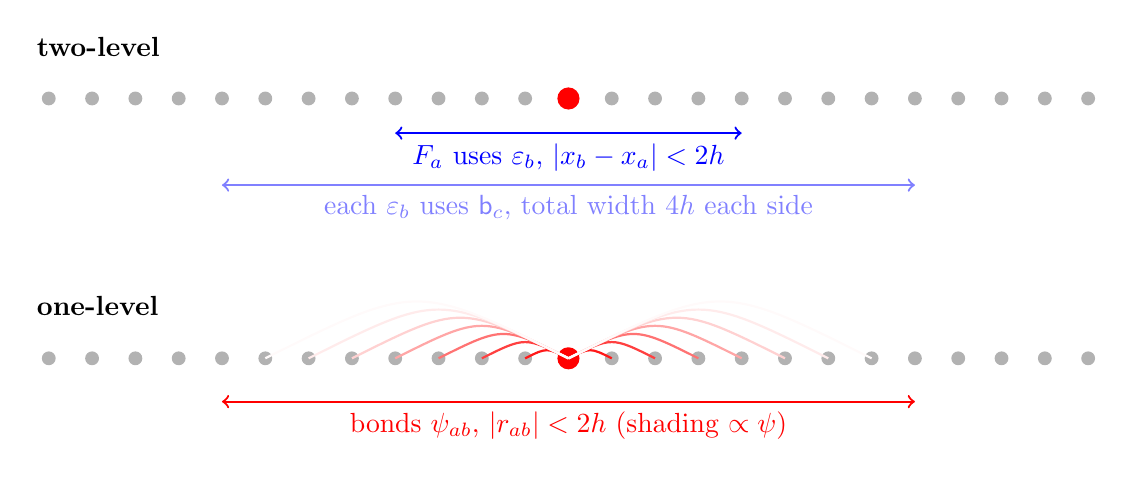
\begin{tikzpicture}[x=0.55cm,y=0.55cm]
  % two-level
  \node[anchor=west] at (-12.5,3.2) {\textbf{two-level}};
  \foreach \i in {-12,...,12} \fill[gray!60] (\i,2) circle (2.5pt);
  \fill[red] (0,2) circle (4pt);
  \draw[blue,thick,<->] (-4,1.2) -- (4,1.2) node[midway,below] {$F_a$ uses $\varepsilon_b$, $|x_b-x_a|<2h$};
  \draw[blue!50,thick,<->] (-8,0.0) -- (8,0.0) node[midway,below] {each $\varepsilon_b$ uses $\bbeta_c$, total width $4h$ each side};
  % one-level
  \node[anchor=west] at (-12.5,-2.8) {\textbf{one-level}};
  \foreach \i in {-12,...,12} \fill[gray!60] (\i,-4) circle (2.5pt);
  \fill[red] (0,-4) circle (4pt);
  \foreach \i/\o in {1/90,2/75,3/55,4/35,5/18,6/8,7/2} {
     \draw[red!\o!white,thick] (0,-4) .. controls (\i/2,-4+0.25*\i) .. (\i,-4);
     \draw[red!\o!white,thick] (0,-4) .. controls (-\i/2,-4+0.25*\i) .. (-\i,-4);}
  \draw[red,thick,<->] (-8,-5.0) -- (8,-5.0) node[midway,below] {bonds $\psi_{ab}$, $|r_{ab}|<2h$ (shading $\propto\psi$)};
\end{tikzpicture}
\caption{Stencils for $h/a=4$.  The two-level force on particle $a$ (red)
depends on $\bbeta$ out to $4h$ through two nested SPH sums.  The one-level
force is a sum of direct pair forces out to $2h$, weighted by $\psi$.}
\label{fig:stencil}
\end{figure}

%=============================================================================
\section{Two dimensions}
\label{sec:twod}

We now repeat the construction in two dimensions, again for a fluid at rest.
The new feature is that $\bbeta$ is a vector and its gradient is a tensor.  We
first try the direct generalization of the 1D bond form and identify what goes
wrong (\Sect{sec:plain2d}).  We then fix it by subtracting a mean-field rotation
and dilation from each bond (\Sect{sec:mf2d}).  To keep the argument simple we
assume throughout that every particle's neighbourhood is isotropic, as on a
perfect hexagonal lattice.  General arrangements are treated in
Ref.~\cite{ParticleMetrics}.

\subsection{The continuum target}

Write the velocity gradient as the matrix $\nabla\bbeta$ with components
\st
\nabla_j\beta_i=\partial_j\beta_i\qquad(\text{row }i,\ \text{column }j),
\stp
so that along a bond
\st
\bbeta(\bm x+\bm r)-\bbeta(\bm x)\simeq(\nabla\bbeta)\,\bm r .
\stp
Split it into its symmetric part $S$,
its antisymmetric part $\Omega$ (the local rotation, i.e.\ the vorticity), and
its trace $\theta$ (the dilation):
\st
S=\tfrac12\big(\nabla\bbeta+(\nabla\bbeta)^T\big),\qquad \Omega=\tfrac12\big(\nabla\bbeta-(\nabla\bbeta)^T\big),\qquad \theta=\nabla\!\cdot\!\bbeta .
\label{split}
\stp
We work in $d$ dimensions, the dimension of both the fluid and the
simulation; the equations hold in 2D and in 3D.  A simulation that resolves
fewer directions than the fluid has, such as planar flow of a 3D fluid, is
treated in Appendix~\ref{sec:unresolved}.
The dissipative function at rest is
\st
K=\frac12\int d^dx\;T\big[\,2\eta\,\mathring S{:}\mathring S+\zeta\,\theta^2\big],
\qquad \mathring S=S-\frac{\theta}{d}\,\one ,
\label{K2dcont}
\stp
with $\mathring S$ traceless.  Two features matter:
\begin{itemize}
\item two independent coefficients, the shear viscosity $\eta$ and the bulk
  viscosity $\zeta$;
\item $\Omega$ does not appear: a rigid rotation costs nothing.  This is what makes
  the viscous force conserve angular momentum;
\end{itemize}
A transverse (shear) wave and a longitudinal wave decay at
\st
\Gamma_T=\frac{\eta}{w}k^2,\qquad
\Gamma_L=\frac{1}{w}\Big[2\eta\,\frac{d-1}{d}+\zeta\Big]k^2 .
\label{Gphys2d}
\stp

\subsection{Plain bond form and its two problems}
\label{sec:plain2d}

The direct generalization of \Eq{K1L} squares the vector bond differences
$\Delta\bbeta_{ab}$:
\st
K_{\rm plain}=\frac12\sum_aV_aT_a\eta_a\sum_{b\neq a}w_{ab}\,
|\Delta\bbeta_{ab}|^2,\qquad
\sum_{b\neq a}w_{ab}\,\bm r_{ab}\bm r_{ab}^T=\one .
\label{Kplain}
\stp
with $w_{ab}$ defined as in 1D.  The second equation is the isotropy
assumption; it fixes $n_a$, the 2D analogue of the 1D bond moment.  For a linear
field the bond differences are exact, so
\st
\sum_bw_{ab}|(\nabla\bbeta)\bm r_{ab}|^2=\nabla_j\beta_i\,\nabla_k\beta_i\sum_bw_{ab}r^j_{ab}r^k_{ab}
=\nabla\bbeta{:}\nabla\bbeta=S{:}S+\Omega{:}\Omega ,
\stp
and
\st
K_{\rm plain}\;\to\;\frac12\int d^dx\;T\eta\,\big[S{:}S+\Omega{:}\Omega\big].
\label{Kplaincont}
\stp
Compare with \Eq{K2dcont}.  There are two problems.
\begin{enumerate}
\item \emph{Rotation is dissipated.}  $\Omega$ appears.  A rigid rotation has
  $S=0$ but $K_{\rm plain}\neq0$.  Microscopically, the pair force is along
  $\Delta\bbeta_{ab}$, not along $\bm r_{ab}$.  It exerts a
  torque, and angular momentum is not conserved.
\item \emph{Only one viscosity.}  There is a single coefficient, so the
  bulk viscosity cannot be set independently of the shear viscosity.  A
  transverse wave happens to come out right: its gradient is half shear, half
  rotation, and the two errors compensate.  But a longitudinal wave
  ($\Omega=0$, $S{:}S=k^2$) decays at $\eta k^2/w$.  Comparing with
  \Eq{Gphys2d}, the plain form has the fixed bulk viscosity
  \st
  \zeta_{\rm plain}=-\frac{d-2}{d}\,\eta ,
  \stp
  which is zero in 2D.
\end{enumerate}
Keeping only the component of the bond difference along the bond, the
central form of DPD, cures the first problem but not the second.
That form ties $\zeta$ to $\eta$ (the Cauchy relation).  With bond differences
alone, both problems cannot be fixed at once.

\subsection{Mean-field form: subtract the local rotation and dilation}
\label{sec:mf2d}

The cure is simple: before squaring a bond difference, subtract the part of it
due to the local rotation and dilation at particle $a$.

\paragraph{The mean field.}  Define the gradient at particle $a$ as the linear
field that best fits its own bond differences, with the same weights as the
bonds:
\st
(\nabla\bbeta)_a\equiv\arg\min_{G}\;\sum_{b\neq a}V_b\,\psi_{ab}\,\big|\Delta\bbeta_{ab}-G\,\bm r_{ab}\big|^2 .
\label{Gmin}
\stp
Setting the derivative with respect to $G$ to zero gives
\st
(\nabla\bbeta)_a\sum_{b\neq a}V_b\,\psi_{ab}\,\bm r_{ab}\bm r_{ab}^T
=\sum_{b\neq a}V_b\,\psi_{ab}\,\Delta\bbeta_{ab}\,\bm r_{ab}^T .
\stp
With the isotropy assumption the bond moment on the left is $n_a\one$, so
\st
(\nabla\bbeta)_a=\sum_{b\neq a}w_{ab}\,\Delta\bbeta_{ab}\,\bm r_{ab}^T .
\label{Ga}
\stp
Split it as in \Eq{split}:
\st
\Omega_a=\tfrac12\big((\nabla\bbeta)_a-(\nabla\bbeta)_a^T\big),\qquad \theta_a=(\nabla\!\cdot\!\bbeta)_a .
\label{Omegaa}
\stp
For a linear field every bond is fitted exactly, and the fit is the true
gradient.  With $\psi=-W'/r$, \Eq{Ga} is the usual SPH gradient.  The minimization form \Eq{Gmin}, however, makes
sense for any $\psi$.
We call $\Omega_a$ and $\theta_a$ mean-field quantities: each is an average over
the neighbourhood of $a$.

\paragraph{Subtract.}  Replace $\Delta\bbeta_{ab}$ by
\st
\mathcal D_{ab}\bbeta=\Delta\bbeta_{ab}-\Big(\Omega_a+\frac{\theta_a}{d}\one\Big)\bm r_{ab},
\label{Dab}
\stp
the \emph{covariant bond difference}.  It vanishes when $\bbeta$ is, around $a$,
a rigid rotation plus a dilation, i.e.\ a conformal Killing field: $\Omega_a$
and $\theta_a$ act as local rotation and Weyl connections
(Appendix~\ref{app:variational}).  Put the bulk viscosity back in an explicit term:
\st
\boxed{\;K=\sum_aV_aT_a\eta_a\sum_{b\neq a}w_{ab}\,
|\mathcal D_{ab}\bbeta|^2+\frac12\sum_aV_aT_a\zeta_a\,\theta_a^2 .\;}
\label{KMF}
\stp

\paragraph{Why it works.}
\begin{itemize}
\item \emph{Continuum limit.}  For a linear field,
  \st
  \mathcal D_{ab}\bbeta=\Big(\nabla\bbeta-\Omega-\frac{\theta}{d}\one\Big)\bm r_{ab}=\Big(S-\frac{\theta}{d}\one\Big)\bm r_{ab},
  \stp
  and the bond sum gives
  \st
  \sum_{b\neq a}w_{ab}\,|\mathcal D_{ab}\bbeta|^2=\tr\Big[\Big(S-\frac{\theta}{d}\one\Big)^2\Big].
  \stp
  This is $\mathring S{:}\mathring S$, and with the $\zeta$ term \Eq{KMF} reduces
  exactly to \Eq{K2dcont}.  Both viscosities are now correct and
  independent.
\item \emph{Rotation.}  For a rigid rotation the fit is $\Omega_a$ and
  $\theta_a=0$, so every covariant bond difference vanishes and $K=0$.  Angular
  momentum is conserved.
\item \emph{Unresolved modes.}  For a mode on the scale of the lattice, the fit
  \Eq{Ga} sees almost nothing.  The subtraction switches off, and
  $K$ reduces to the plain bond form.  That form has no null modes
  (it is positive for every non-constant $\bbeta$), so short wavelengths are still damped.
\end{itemize}

\paragraph{Resolved plus residual.}  The argument above used linear fields.
For a general field, split each bond difference into the part that the fit
explains and the rest,
\st
\Delta\bbeta_{ab}=(\nabla\bbeta)_a\,\bm r_{ab}+\bm\delta_{ab} .
\label{resid}
\stp
The residual $\bm\delta_{ab}$ is what the fit misses.  It vanishes for a linear
field, is of order the curvature of $\bbeta$ across the star for a smooth field,
and is nearly all of $\Delta\bbeta_{ab}$ for an unresolved mode.  Because
$(\nabla\bbeta)_a$ is a least-squares fit, the residuals are orthogonal to the
bond vectors; this is the condition that defines the minimum in \Eq{Gmin}:
\st
\sum_{b\neq a}w_{ab}\,\bm\delta_{ab}\,\bm r_{ab}^T=0 .
\label{orthog2d}
\stp
The subtraction in \Eq{Dab} is linear in $\bm r_{ab}$, so
\st
\mathcal D_{ab}\bbeta=\Big(S_a-\frac{\theta_a}{d}\one\Big)\bm r_{ab}+\bm\delta_{ab},
\stp
with $S_a$ the symmetric part of the fit.  When this is squared and summed
with $w_{ab}$, the cross term is proportional to \Eq{orthog2d} and vanishes, and
the isotropy condition of \Eq{Kplain} turns the first term into a trace.
$K$ splits exactly into two non-negative pieces:
\st
K=\underbrace{\frac12\sum_aV_aT_a\big[2\eta\,\mathring S_a{:}\mathring S_a+\zeta\,\theta_a^2\big]}_{\text{resolved}}
+\underbrace{\sum_aV_aT_a\eta_a\sum_{b\neq a}w_{ab}\,|\bm\delta_{ab}|^2}_{\text{residual}} .
\label{split2d}
\stp
\begin{itemize}
\item The \emph{resolved} term is the continuum dissipative function
  \Eq{K2dcont} evaluated on the fitted gradient.  It is a two-level form, with
  the fit in place of the SPH gradient.
\item The \emph{residual} term is what the bonds add.  It is zero for linear
  fields and small for smooth ones, so it does not change the continuum limit.
  It is what damps the modes the fit cannot see.
\end{itemize}
The split is an identity, valid for any field; it only requires that the fit be
computed with the same weights as the bonds.  Ref.~\cite{ParticleMetrics}
proves it on general arrangements.

In 1D none of this is needed: there is no rotation and a single coefficient
$\kappa$, so the plain form \Eq{K1L} is already right.

\subsection{Viscous forces}
\label{sec:force2d}

The viscous force on particle $a$ is minus the derivative of the dissipative
function, as in \Eq{generic}:
\st
\bm F_a=-\frac{\partial K}{\partial\bbeta_a} .
\stp
$K$ depends on $\bbeta$ in two ways.  It depends explicitly on the bond
differences $\Delta\bbeta_{ab}$ in $\mathcal D_{ab}\bbeta$.  And it depends
implicitly on the neighbours' $\bbeta$ through the mean fields $\Omega_a$ and
$\theta_a$, which are computed from the fit.  The force therefore has two parts,
\st
\bm F_a=\bm F_a^{\rm bond}+\bm F_a^{\rm MF} .
\stp
The bond force is the derivative at fixed mean fields; the mean-field force is
the chain rule through the mean fields.  We take them in turn.  On a general
arrangement the weights are the corrected weights of
Ref.~\cite{ParticleMetrics}, so that the isotropy condition of \Eq{Kplain}
holds exactly; everything below then holds on any arrangement.

\paragraph{Bond forces.}  Write $K=\sum_aK_a$, with $K_a$ the contribution of
particle $a$.  As in 1D, \Eq{tab}, define for each bond the traction
\st
\tf_{ab}=-\frac{\partial K_a}{\partial\Delta\bbeta_{ab}}\Big|_{\rm MF}
=-2V_aT_a\eta_a\,w_{ab}\,\mathcal D_{ab}\bbeta ,
\label{tab2d}
\stp
the momentum given by $a$ to $b$ along the bond $ab$.  It is now a vector, and
need not point along the bond.  Along the same bond $b$ gives $\tf_{ba}$ to
$a$, so the bond force is a sum of antisymmetric pair forces, as in \Eq{Fa}:
\st
\bm F_a^{\rm bond}=\sum_{b\neq a}\bm f_{ab},\qquad
\bm f_{ab}=-(\tf_{ab}-\tf_{ba})=-\bm f_{ba} .
\stp
For a linear field the traction is a momentum flux times a face area, as in
\Eq{tface}:
\st
\tf_{ab}=\Pi_a\,\bm A_{ab},\qquad
\Pi_a=-2T_a\eta_a\Big(S_a-\frac{\theta_a}{d}\one\Big),\qquad
\bm A_{ab}=V_a\,w_{ab}\,\bm r_{ab} .
\stp
The faces close,
\st
\sum_{b\neq a}\bm A_{ab}\bm r_{ab}^T=V_a\one .
\stp
As in \Eq{virial}, for a
general field we define the stress of particle $a$ by the virial of its faces,
\st
V_a\Pi_a=\sum_{b\neq a}\tf_{ab}\,\bm r_{ab}^T ,
\label{virial2d}
\stp
which for a linear field is the expression above.

\paragraph{The rotation exerts no mean-field force.}  Define the rotation
\emph{variationally}, as the local rigid rotation that minimizes the
particle's dissipation:
\st
\Omega_a=\arg\min_{\Omega'\in\text{antisym}}\;\sum_{b\neq a}w_{ab}
\Big|\Delta\bbeta_{ab}-\Big(\Omega'+\frac{\theta_a}{d}\one\Big)\bm r_{ab}\Big|^2 .
\label{Omegavar}
\stp
The minimizer is exactly the antisymmetric part of the fit
(Appendix~\ref{app:variational}), so \Eq{Omegaa} is unchanged; it has merely
been given a variational meaning.  The payoff is in the chain rule.  The
force through the rotation is
\st
-\sum_b\frac{\partial K}{\partial\Omega_b}{:}\frac{\partial\Omega_b}{\partial\bbeta_a}=0 ,
\stp
because at the minimum the derivative of $K$ with respect to each $\Omega_b$
vanishes.  (This is the envelope theorem: the total derivative of $K$ equals
the partial derivative at fixed $\Omega$.)  The rotation therefore produces
\emph{no} mean-field force.  The stationarity condition itself says that the
faces of each particle carry no net torque, i.e.\ that the stress of each
particle is symmetric:
\st
\sum_{b\neq a}\bm r_{ab}\times\tf_{ab}=0,\qquad \Pi_a=\Pi_a^T .
\stp

\paragraph{The dilation force.}  Only the dilation, which is not variational,
carries a mean-field force.  Writing $G_a=(\nabla\bbeta)_a$ for short, the chain
rule through $\theta_a=\tr G_a$ gives
\st
\bm F^{\rm MF}_a=-\sum_bE_b{:}\frac{\partial G_b}{\partial\bbeta_a},\qquad
E_a=\frac{\partial K}{\partial G_a}=V_a\Big(T_a\zeta_a\,\theta_a+\frac{\tr\Pi_a}{d}\Big)\one .
\label{fMF}
\stp
The first term of $E_a$ is from the bulk term of $K$.  The second is from
the dilation subtracted in every bond, and involves the stress \Eq{virial2d}.  From \Eq{Ga}, the derivative of the fit is
\st
\frac{\partial G_{b,ij}}{\partial\bbeta_{a,k}}=\delta_{ik}\,w_{ba}\,r^j_{ba}\quad(b\neq a),\qquad
\frac{\partial G_{a,ij}}{\partial\bbeta_{a,k}}=-\delta_{ik}\sum_{b\neq a}w_{ab}\,r^j_{ab}.
\stp
Thus each neighbour of $a$ (for instance particle $b$) exerts a force
\st
\bm F^{\rm MF}_a=\sum_{b\neq a}\bm f^{\rm MF}_{ab},\qquad
\bm f^{\rm MF}_{ab}=\big(w_{ab}E_a+w_{ba}E_b\big)\,\bm r_{ab}=-\bm f^{\rm MF}_{ba},
\stp
directed along the bond.  It is antisymmetric, so momentum is conserved.  (Had
$\Omega_a$ been defined non-variationally, for instance from the SPH gradient,
$\Pi_a$ would not be symmetric, and an extra torque term, proportional to the
antisymmetric part of $\Pi_a$, would appear in $E_a$.  The same happens on
particles where the $\Lambda$ correction fails.)

%=============================================================================
\section{A moving fluid in two dimensions}
\label{sec:moving2d}

We now let the background move with a velocity $\bm v$.  The
construction of \Sect{sec:mf2d} carries over with three substitutions:
\begin{itemize}
\item bonds are measured by their length in the rest frame of the particle;
\item bond differences are contracted with the comoving metric $\ell$ instead of $\delta$;
\item the scalar part of the strain is removed along the projector $P$ instead of $\one/d$.
\end{itemize}
The rotation is subtracted as before.

\subsection{Thermodynamic variables}

For a moving fluid the derivative of the energy with respect to the particle
entropy is not the rest-frame temperature $T$.  At fixed momentum it is
$T/\gamma$, so
\st
\frac{\partial H}{\partial s_a}=\frac{T_a}{\gamma_a},\qquad
\gamma_a=\frac{1}{\sqrt{1-v_a^2}},\qquad
\bbeta_a=\frac{\dot{\bm x}_a}{\partial H/\partial s_a}=\frac{\gamma_a\bm v_a}{T_a}=\frac{\bm u_a}{T_a}.
\stp
So $\bbeta$ is the spatial part of the thermal vector $\beta^\mu=u^\mu/T$.  At
rest the two temperatures coincide.  From here on $T$ is the rest-frame
temperature.

\subsection{The continuum target}

In the density frame the viscous stress is
\st
\Pi^{ij}=-T\kappa^{ijmn}S_{mn},\qquad S_{ij}=\partial_{(i}\beta_{j)},
\stp
and the dissipative function is
\st
K=\frac12\int d^dx\;T\kappa^{ijmn}S_{ij}S_{mn}
\label{Kv}
\stp
(Ref.~\cite{BhambureSinghTeaney2025}).  The tensor $\kappa^{ijmn}(v)$ is built
from two objects.  The first is the \emph{comoving metric},
\st
\ell^{ij}=\delta^{ij}-v^iv^j,\qquad (\ell^{-1})_{ij}=\delta_{ij}+\gamma^2v_iv_j ,
\stp
the inverse metric of the comoving coordinates.  The second is
the \emph{scalar projector},
\st
P_{ij}=-c_s^2u_iu_j+\frac1d\big(\delta_{ij}+u_iu_j\big),\qquad
\avg{P\ell}\equiv P_{ij}\ell^{ij}=1-c_s^2v^2 ,
\stp
the direction along which the scalar part of the strain is removed.  It
encodes the elimination of time derivatives with the Euler equations and the
change to the density frame.  The shear and bulk parts are
\begin{align}
\kappa_\eta^{ijmn}&=2\eta\Big[\ell^{(im}\ell^{j)n}
 -\frac{\ell^{ij}(\ell P\ell)^{mn}+(\ell P\ell)^{ij}\ell^{mn}}{\avg{P\ell}}
 +\frac{\avg{P\ell P\ell}}{\avg{P\ell}^2}\,\ell^{ij}\ell^{mn}\Big],\\
\kappa_\zeta^{ijmn}&=\zeta\,\frac{\ell^{ij}\ell^{mn}}{\avg{P\ell}^2} .
\end{align}

\paragraph{A comoving norm.}  Define the comoving dilation, which at rest is
$\nabla\!\cdot\!\bbeta$, and the strain with its scalar part removed,
\st
\theta=\frac{\ell^{ij}S_{ij}}{\avg{P\ell}},\qquad
\mathring S_{ij}=S_{ij}-\theta P_{ij} ,
\label{thetadefv}
\stp
so that $\mathring S$ is traceless in the comoving metric.  Then
\st
\tfrac12T\kappa^{ijmn}S_{ij}S_{mn}
=T\eta\,\tr\big(\ell\mathring S\ell\mathring S\big)+\tfrac12T\zeta\theta^2 ,
\label{normid}
\stp
This is the static form \Eq{K2dcont} with $\delta^{ij}\to\ell^{ij}$ and $\theta$
the comoving dilation \Eq{thetadefv}.

\subsection{Bond form}

\paragraph{Comoving distance.}  All positions are taken at the same lab time.
The length of the bond $ab$ in the rest frame of $a$ is
\st
\rho_{ab}^2=\bm r_{ab}^T\,\ell_a^{-1}\,\bm r_{ab}
=r_{ab}^2+\gamma_a^2(\bm v_a\!\cdot\bm r_{ab})^2 ,
\label{comovingdist}
\stp
the projection of the separation $(0,\bm r_{ab})$ orthogonal to $u_a$.  The bond
weight is evaluated at it, $\psi_{ab}=\psi(\rho_{ab})$.  A moving fluid is
Lorentz contracted along $\bm v$; measuring bonds by $\rho_{ab}$ keeps the
stencil round in the rest frame, so each particle has the same neighbours at
every velocity.

\paragraph{Comoving moment.}  Weights that are round in $\rho$ give a bond
moment proportional to $\ell_a$, \EqPM{Mcomoving}.  With the corrected weights
of Ref.~\cite{ParticleMetrics}, \EqPM{Lambdadef}, this holds exactly:
\st
\sum_{b\neq a}w_{ab}\,\bm r_{ab}\bm r_{ab}^T=\ell_a,\qquad
w_{ab}=\frac{V_b\,\psi_{ab}}{n_a} .
\label{wv}
\stp
The face vectors then close on the comoving metric,
\st
\bm A_{ab}=V_aw_{ab}\bm r_{ab},\qquad \sum_{b\neq a}\bm A_{ab}\bm r_{ab}^T=V_a\ell_a .
\stp

\paragraph{Mean field.}  The fit $(\nabla\bbeta)_a$ is defined by \Eq{Gmin}, which
involves no metric.  Its rotation $\Omega_a$ is the antisymmetric part, as at
rest, and its scalar is the comoving dilation,
\st
\Omega_a=\tfrac12\big((\nabla\bbeta)_a-(\nabla\bbeta)_a^T\big),\qquad
\theta_a=\frac{\ell_a^{ij}\,(\nabla_j\beta_i)_a}{\avg{P\ell}_a} .
\label{thetaav}
\stp

\paragraph{Subtract and square.}  The covariant bond difference becomes
\st
\mathcal D_{ab}\bbeta=\Delta\bbeta_{ab}-\big(\Omega_a+\theta_aP_a\big)\bm r_{ab},
\label{Dabv}
\stp
which reduces to \Eq{Dab} at rest.  Contracting it with the comoving metric,
\st
\boxed{\;K=\sum_aV_aT_a\eta_a\sum_{b\neq a}w_{ab}\,
\mathcal D_{ab}\bbeta\cdot\ell_a\cdot\mathcal D_{ab}\bbeta
+\frac12\sum_aV_aT_a\zeta_a\,\theta_a^2 ,\;}
\label{KMFv}
\stp
where
\st
\mathcal D\bbeta\cdot\ell\cdot\mathcal D\bbeta=(\mathcal D\beta)_i\,\ell^{ij}(\mathcal D\beta)_j .
\stp

\paragraph{Why it works.}
\begin{itemize}
\item \emph{Continuum limit.}  For a linear field the fit is exact, and
  \st
  \mathcal D_{ab}\bbeta=\big(\nabla\bbeta-\Omega-\theta P\big)\bm r_{ab}=\mathring S\,\bm r_{ab} .
  \stp
  By \Eq{wv} the bond sum is
  \st
  \sum_{b\neq a}w_{ab}\;\big(\mathring S_{ik}\,r^k_{ab}\big)\;\ell^{ij}\;\big(\mathring S_{jl}\,r^l_{ab}\big)
  =\tr\big(\ell\mathring S\ell\mathring S\big),
  \stp
  and with the $\zeta$ term \Eq{KMFv} reduces exactly to \Eq{normid}.
\item \emph{Rotation.}  A rigid rotation has $S=0$, hence $\theta_a=0$, and every
  covariant bond difference vanishes.
\item \emph{Unresolved modes.}  The fit sees almost nothing, the subtraction
  switches off, and the bond term reduces to a positive plain bond form
  contracted with $\ell_a$.
\end{itemize}

\paragraph{Resolved plus residual.}  The split \Eq{split2d} carries over.  With
the residual of \Eq{resid}, the cross terms vanish for any contraction, since the
orthogonality \Eq{orthog2d} does not involve the metric.  With \Eq{wv},
\st
K=\underbrace{\sum_aV_aT_a\Big[\eta_a\tr\big(\ell_a\mathring S_a\ell_a\mathring S_a\big)+\tfrac12\zeta_a\theta_a^2\Big]}_{\text{resolved}}
+\underbrace{\sum_aV_aT_a\eta_a\sum_{b\neq a}w_{ab}\,\bm\delta_{ab}\cdot\ell_a\cdot\bm\delta_{ab}}_{\text{residual}} ,
\stp
with $\mathring S_a$ built from the fit.  The resolved term is the continuum
\Eq{normid} on the fitted gradient; the residual damps what the fit cannot
see.

\subsection{Viscous forces}
\label{sec:forcev}

As at rest, the force $\bm F_a=-\partial K/\partial\bbeta_a$ has a bond part, the
derivative at fixed mean fields, and a mean-field part, the chain rule through
$\Omega_a$ and $\theta_a$:
\st
\bm F_a=\bm F_a^{\rm bond}+\bm F_a^{\rm MF} .
\stp

\paragraph{Bond forces.}  The traction is defined as in \Eq{tab2d}.  Since
$\mathcal D_{ab}\bbeta$ is now contracted with $\ell_a$, the traction carries an
upper index, raised by $\ell_a$:
\st
\mathsf t^i_{ab}=-\frac{\partial K_a}{\partial(\Delta\beta_{ab})_i}\Big|_{\rm MF}
=-2V_aT_a\eta_a\,w_{ab}\,\ell_a^{ij}(\mathcal D_{ab}\beta)_j ,
\label{tabv}
\stp
the momentum given by $a$ to $b$ along the bond $ab$.  The bond force is again
a sum of antisymmetric pair forces,
\st
\bm F_a^{\rm bond}=\sum_{b\neq a}\bm f_{ab},\qquad
\bm f_{ab}=-(\tf_{ab}-\tf_{ba})=-\bm f_{ba} .
\stp
Because $\rho_{ab}$ and $\ell_a$ use the velocity of $a$, the two ends of a bond
see different weights and $\tf_{ab}\neq-\tf_{ba}$; the pair force is
antisymmetric regardless.  For a linear field the traction is a momentum flux
times a face area,
\st
\mathsf t^i_{ab}=\Pi_a^{ik}A_{ab\,k},\qquad
A_{ab\,k}=(\ell_a^{-1})_{kl}A^l_{ab},\qquad
\Pi_a=-2T_a\eta_a\,\ell_a\mathring S\ell_a ,
\stp
with $A_{ab\,k}$ the face covector of Ref.~\cite{ParticleMetrics}.  This is the
shear stress carried by the bonds; the remainder of the viscous stress, which is
proportional to $\ell^{ij}$, is carried by the mean field.  For a general field the stress of the particle is
again the virial of its faces,
\st
V_a\Pi_a^{ij}=\sum_{b\neq a}\mathsf t^i_{ab}\,r^j_{ab} .
\label{virialv}
\stp

\paragraph{The rotation exerts no mean-field force.}  As at rest
(Appendix~\ref{app:variational}), consider minimizing the bond term over a local
rotation $\Omega'$.  As in \Eq{genid}, only the resolved part depends on
$\Omega'$.  With $M_a=n_a\ell_a$ and the contraction with $\ell_a$ it is
proportional to a Frobenius norm,
\st
\tr\big(\ell X\ell X^T\big)=\big|\ell^{1/2}X\ell^{1/2}\big|^2,\qquad
X=\nabla\bbeta-\theta P-\Omega' .
\stp
It is minimized when
\st
\ell^{1/2}\,\Omega'\,\ell^{1/2}=\text{antisym}\big(\ell^{1/2}\,\nabla\bbeta\,\ell^{1/2}\big),
\stp
since $P$ is symmetric and drops out.  In 2D every antisymmetric matrix is a
multiple of a single matrix $J$, and $BJB=(\det B)\,J$ for symmetric $B$.
Hence the minimizer is
\st
\Omega'=\tfrac12\big(\nabla\bbeta-(\nabla\bbeta)^T\big)=\Omega_a\qquad(\text{2D, any }\bm v),
\stp
the same subtraction as at rest.  (In 3D it is instead the $\ell$-weighted
antisymmetric part.)
So the rotation is variational at any velocity.  The derivative of $K$ with
respect to $\Omega_a$ vanishes at the minimum, so the rotation produces no
mean-field force, and the stationarity condition says that the
faces carry no net torque: $\Pi_a$ of \Eq{virialv} is symmetric.

\paragraph{The dilation force.}  Only the dilation, which is not variational,
carries a mean-field force.  Writing $G_a=(\nabla\bbeta)_a$,
the chain rule goes through
\st
\frac{\partial\theta_a}{\partial G_{a,ij}}=\frac{\ell^{ij}_a}{\avg{P\ell}_a},
\stp
and gives
\st
E_a=\frac{\partial K}{\partial G_a}=e_a\,\ell_a,\qquad
e_a=\frac{V_a}{\avg{P\ell}_a}\Big(T_a\zeta_a\,\theta_a+P_{a,ij}\,\Pi_a^{ij}\Big).
\label{Eav}
\stp
The first term is from the bulk term of $K$; the second is from the
dilation subtracted in every bond.  At rest this reduces to the $E_a$ of
\Eq{fMF}.  With the corrected weights the fit carries a factor $\ell_b^{-1}$,
\st
G_b=\sum_{c\neq b}w_{bc}\,\Delta\bbeta_{bc}\,\bm r_{bc}^T\,\ell_b^{-1},
\stp
which cancels the $\ell_b$ in $E_b$.  Thus each
neighbour of $a$ (for instance particle $b$) exerts a central force,
\st
\bm F^{\rm MF}_a=-\sum_bE_b{:}\frac{\partial G_b}{\partial\bbeta_a}
=\sum_{b\neq a}\bm f^{\rm MF}_{ab},\qquad
\bm f^{\rm MF}_{ab}=\big(w_{ab}\,e_a+w_{ba}\,e_b\big)\,\bm r_{ab}=-\bm f^{\rm MF}_{ba} .
\label{fMFv}
\stp
It is directed along the bond and antisymmetric, so momentum is conserved.

%=============================================================================
\section{Implementation}
\label{sec:impl}

This section outlines how the viscous force of \Sect{sec:moving2d} is computed
in the code (\texttt{dissipative\_force!}, which calls
\texttt{\_bond\_dissipation!} in \texttt{src/celllist.jl}).  The fluid at rest is
the special case $\bm v_a=0$.  The routine accumulates the gradient
\st
\bm g_a=\frac{\partial K}{\partial\bbeta_a}
\stp
and returns the force $\bm F_a=-\bm g_a$.

\paragraph{Organization.}  There is a single loop over particles.  Each particle
$a$ builds its own star of neighbours, computes its weights and its mean
field, and then distributes its contributions to $\bm g$ over the star.  Both
the bond force and the mean-field force of particle $a$ reach only the
particles of its own star, so the stencil is $2h$, as in 1D.  The ordering of
the loop does not matter, because every contribution enters $\bm g$ in
equal and opposite pairs.

\medskip
\noindent\fbox{\begin{minipage}{0.95\textwidth}
\textbf{Algorithm: viscous force} $\bm F_a=-\partial K/\partial\bbeta_a$
\begin{algorithmic}[1]
\State $\bm g_a\gets0$ for all $a$
\For{each particle $a$}
  \State \textbf{star}: all $b\neq a$ with $|\bm r_{ab}|<2h$ (minimum image)
  \State \textbf{local data}: $V_a$, $T_a$, $\eta_a$, $\zeta_a$, and $\ell_a$, $\ell_a^{-1}$, $P_a$, $\avg{P\ell}_a$ from $\bm v_a$
  \State \textbf{bare weights}: $\psi_{ab}$ at the comoving distance \Eq{comovingdist}
  \State \textbf{correction}: solve the $4\times4$ system \EqPM{Lambdadef} for $\Lambda_a$ and $n_a$
  \If{a corrected weight is negative} \State fall back to $\Lambda_a=0$ \EndIf
  \State \textbf{weights}: $w_{ab}$ of \Eq{wv}
  \State \textbf{fit}: bond moment $M_a$ and $G_a=(\nabla\bbeta)_a$ by \Eq{Gmin}
  \State \textbf{mean field}: $\Omega_a$ and $\theta_a$ by \Eq{thetaav}
  \For{each $b$ in the star} \Comment{bond force}
    \State $\mathcal D_{ab}\bbeta$ by \Eq{Dabv}, traction $\tf_{ab}$ by \Eq{tabv}
    \State $\bm g_a\gets\bm g_a+\tf_{ab}$, \quad $\bm g_b\gets\bm g_b-\tf_{ab}$
    \State $V_a\Pi_a\gets V_a\Pi_a+\tf_{ab}\,\bm r_{ab}^T$ \Comment{virial \Eq{virialv}}
  \EndFor
  \State \textbf{mean-field stress}: $E_a=e_a\ell_a$ by \Eq{Eav}
  \For{each $b$ in the star} \Comment{mean-field force}
    \State $\bm q_{ab}=V_b\psi_{ab}\,E_aM_a^{-1}\bm r_{ab}$
    \State $\bm g_b\gets\bm g_b+\bm q_{ab}$, \quad $\bm g_a\gets\bm g_a-\bm q_{ab}$
  \EndFor
\EndFor
\State $\bm F_a\gets-\bm g_a$ for all $a$
\end{algorithmic}
\end{minipage}}
\medskip

\paragraph{Remarks.}
\begin{itemize}
\item \emph{Bond force.}  Particle $a$ gives $\tf_{ab}$ to $b$, so it is added
  to the force on $b$ and subtracted from the force on $a$.  The traction of
  the reverse bond is added when the loop reaches $b$.  Together they give the
  pair force of \Eq{tabv}.
\item \emph{Mean-field force.}  The vector $\bm q_{ab}$ is the derivative of the
  dilation term of particle $a$ with respect to $\bbeta_b$, through the fit.
  It is written with the full $M_a^{-1}$, so it remains correct when the
  $\Lambda$ correction falls back.  When the correction succeeds,
  $M_a=n_a\ell_a$, and $\bm q_{ab}$ reduces to the central force of
  \Eq{fMFv}.
\item \emph{Torque term.}  The code also adds to $E_a$ a term proportional to
  the antisymmetric part of $\Pi_a$.  It vanishes whenever the correction
  succeeds, since the rotation is then variational, and it keeps the force
  exact on fallback particles.
\item \emph{One dimension.}  The 1D path has no mean field.  It uses a plain
  bond term with the full $T\kappa$ on the bonds.
\item \emph{Unresolved dimensions.}  For planar flow of a 3D fluid the code
  currently uses $d=3$ in $P$ and in the subtracted dilation, and puts the
  out-of-plane shear into the coefficient of $\theta^2$.  This is an equally
  exact split for linear fields; Appendix~\ref{sec:unresolved} uses $d=2$ with
  $\zeta_{\rm eff}$.
\end{itemize}

\paragraph{Use in the dissipative step.}  The force updates the momenta at
fixed positions, and the entropy follows from \Eq{generic}:
\st
\Delta\bm m_a=\Delta t\,\bm F_a,\qquad
\Delta s_a=-\bbeta_a\cdot\Delta\bm m_a .
\stp
The total entropy grows by $2K\,\Delta t$, and the total momentum is unchanged.

%=============================================================================
\section{Summary and outlook}
\label{sec:summary}

\begin{enumerate}
\item In one dimension at rest, the one-level form \Eq{K1L} is the graph
  Laplacian of $\bbeta$ with weights $w_{ab}$.  It is normalized so that
  linear profiles are exact on any arrangement.  Its force is a sum of
  momentum-conserving pair forces, the differences of the tractions $\mathsf t_{ab}$,
  and each bond produces entropy.
\item The two-level form sees $\bbeta$ only through a smoothed gradient, and
  patterns that gradient misses, such as the zigzag, are not damped.  The
  bond form has $\bbeta=$ const as its only zero mode.
\item In 2D the plain bond form dissipates rotation and has only one
  viscosity.  Subtracting the mean-field rotation $\Omega_a$ and dilation
  $\theta_a$, taken from the least-squares fit, fixes both.  The rotation is
  variational: the stress of each particle is symmetric and the rotation exerts
  no mean-field force.  The dilation carries the bulk viscosity and a central
  mean-field force.  For unresolved modes the subtraction switches off, so they
  remain damped.
\item For a moving fluid the same form holds with the comoving distance, the
  comoving metric $\ell$, and the scalar removed along $P$.  Its continuum limit
  is the density-frame $\kappa^{ijmn}(v)$, and in 2D the subtracted rotation is
  the same as at rest.
\end{enumerate}

\paragraph{Noise.}  The one-level form has an obvious fluctuating partner.
$K_{1L}$ is a sum over bonds, \Eq{Kpairs}, so the fluctuation--dissipation
theorem asks for independent noise on each bond,
\st
\delta m_a=\sum_{b\neq a}\sqrt{2c_{ab}\,\Delta t}\;\xi_{ab},\qquad
\xi_{ab}=-\xi_{ba},\quad\langle\xi_{ab}^2\rangle=1 ,
\stp
i.e.\ random tractions on the faces, as in dissipative particle dynamics and
the smoothed DPD of Ref.~\cite{EspanolRevenga2003}.  The two-level noise is
instead the SPH divergence of a per-particle random stress, and it shares the
null mode.  In 2D the noise must also respect the no-torque constraint
(Appendix~\ref{app:variational}).


%=============================================================================
\appendix
\section{Variational form of the mean field}
\label{app:variational}

This appendix shows that the subtracted rotation of \Sect{sec:mf2d} is a
minimizer of $K$ itself.  This has practical consequences for the force and for
the noise.  We work in 2D with particle $a$ fixed, and drop the label $a$ where
it is unambiguous.

\subsection{The rotation is a minimizer of $K$}

Replace the subtraction in \Eq{Dab} by a general linear one, $A\bm r_{ab}$.  As
in \Eq{split2d}, the residual does not depend on $A$, and the bond sum of
particle $a$ splits as
\st
\sum_{b\neq a}w_{ab}\big|\Delta\bbeta_{ab}-A\bm r_{ab}\big|^2
=\tr\big[(\nabla\bbeta-A)(\nabla\bbeta-A)^T\big]+\sum_{b\neq a}w_{ab}|\bm\delta_{ab}|^2 .
\label{genid}
\stp
The Frobenius norm splits orthogonally into symmetric and antisymmetric parts.
Subtracting a rotation $\Omega'$ and the dilation,
\st
A=\Omega'+\frac{\theta}{d}\one,\qquad
\tr\big[(\nabla\bbeta-A)(\nabla\bbeta-A)^T\big]
=\Big|S-\frac{\theta}{d}\one\Big|^2+\big|\Omega-\Omega'\big|^2 .
\stp
The bond term of $K$, and therefore $K$ itself (the bulk
term does not involve $\Omega'$), is minimized by $\Omega'=\Omega_a$:
\st
\boxed{\;\Omega_a=\arg\min_{\Omega'\,\in\,\text{antisym}}\;
\sum_{b\neq a}V_b\psi_{ab}\Big|\Delta\bbeta_{ab}-\Big(\Omega'+\frac{\theta_a}{d}\one\Big)\bm r_{ab}\Big|^2 .\;}
\label{Omegamin}
\stp
Subtracting the fitted rotation is therefore the same as letting each particle
choose the local rigid rotation that minimizes its dissipation.  In convex
language, $K$ is an \emph{infimal convolution} over local rotations.
This is the operation dual, under Legendre transform, to adding a constraint;
the rotation is the Lagrange multiplier that enforces zero torque on the
tractions.  Two
consequences follow.

\paragraph{1. No net torque.}  The stationarity condition of \Eq{Omegamin} is
\st
\Pi_a=\Pi_a^T,\qquad
V_a\Pi_a=\sum_{b\neq a}\tf_{ab}\,\bm r_{ab}^T,\quad
\tf_{ab}=-2V_aT_a\eta_a\,w_{ab}\,\mathcal D_{ab}\bbeta.
\stp
In 2D the antisymmetric part of the virial is the torque of the tractions about
$a$.  The faces of each particle carry \emph{no net
torque} about it, for any $\bbeta$ field, not just a rigid rotation.

\paragraph{2. No rotational mean-field force.}  The derivative of $K$ with
respect to $\Omega_a$ vanishes at the minimum, so the total derivative of $K$
with respect to $\bbeta$ equals the partial derivative at fixed $\Omega_a$ (the
envelope theorem).  The chain-rule force through $\Omega_a$, which
would be proportional to the antisymmetric part of $\Pi_a$, vanishes identically.  Only
the dilation carries a mean-field force:
\st
E_a=V_a\Big(T_a\zeta_a\,\theta_a+\frac{\tr\Pi_a}{d}\Big)\one .
\stp

\subsection{Rotation and dilation as connections}

For a linear field the covariant bond difference \Eq{Dab} is the traceless
strain applied to the bond, i.e.\ the conformal Killing operator.  Its kernel is the rigid rotations and dilations.  Subtracting the rotation compares $\bbeta_b$ with $\bbeta_a$ after a local rotation:
$\Omega_a$ is a linearized rotation connection at $a$.  Minimizing over it,
\Eq{Omegamin}, integrates the connection out, and its equation of motion is the
no-torque condition.  The subtracted dilation is likewise a Weyl
connection, as in the Weyl-covariant form of conformal
hydrodynamics~\cite{Loganayagam2008}.  Weyl rescaling, however, is a symmetry of
the shear part only, and the bulk viscosity breaks it.  That is why $\theta_a$
cannot be integrated out and the bulk term is added explicitly.  Unlike
lattice gauge fields, $\Omega_a$ and $\theta_a$ belong to the particle, not to
the bond.

\subsection{Dual picture and the noise}

The Legendre dual of the dissipative function is the dissipation potential in
terms of forces.  Under this duality the infimum over local rotations in
\Eq{Omegamin} becomes a constraint on the tractions: the faces of each
particle must carry no net torque.  For the stochastic scheme this suggests the
form of the noise.  Draw an independent random traction $\delta\tf_{ab}$ on each
face, as in DPD, and project it onto the torque-free subspace around each
particle.  In the grid scheme~\cite{BhambureSinghTeaney2025} the noise is instead a
tensor $\xi^{ij}$ at the cell corners, contracted with the wall areas
$d\Sigma_j$; on particles the faces are the primary objects, and the noise has
one index.  The dilation, which is not variational, needs its own explicit mean-field noise of
strength set by $\zeta$.


%=============================================================================
\section{Unresolved dimensions}
\label{sec:unresolved}

In the main text $d$ is the dimension of both the fluid and the simulation.
Here we separate the two.  Let
\begin{itemize}
\item $d$ be the dimension of the fluid, which fixes the traceless strain and
  the projector $P$;
\item $d_s\le d$ be the dimension of the simulation, the number of directions
  that are resolved.
\end{itemize}
Nothing varies along the other $d-d_s$ directions, and the velocity lies in
the resolved ones.  An example is planar flow of a three-dimensional fluid,
$d=3$ and $d_s=2$.  Write $\tr_d$ for a trace over all $d$ directions and
$\tr_{d_s}$ for a trace over the resolved ones only.  The bonds see only the
resolved components, so the bond construction produces $\tr_{d_s}$, while the
dissipative function of the fluid is a $\tr_d$.

\paragraph{The result.}  Everything in the main text can be used with
$d\to d_s$, i.e.\ as for a $d_s$-dimensional fluid, provided the bulk viscosity
is replaced by
\st
\boxed{\;\zeta\;\to\;\zeta_{\rm eff}=\zeta+2\eta\,\varepsilon,\qquad
\varepsilon=\frac1{d_s}-\frac1d .\;}
\label{zetaeff}
\stp
For $d=3$ and $d_s=2$, $\varepsilon=1/6$ and $\zeta_{\rm eff}=\zeta+\eta/3$.

\paragraph{At rest.}  The strain $S$ has components only in the resolved
directions, with trace $\theta$.  The traceless strain of the fluid and of the
simulation are
\st
\mathring S_d=S-\frac{\theta}{d}\one_d,\qquad
\mathring S_{d_s}=S-\frac{\theta}{d_s}\one_{d_s} .
\stp
Their norms are
\st
\tr_d\big(\mathring S_d\mathring S_d\big)=S{:}S-\frac{\theta^2}{d},\qquad
\tr_{d_s}\big(\mathring S_{d_s}\mathring S_{d_s}\big)=S{:}S-\frac{\theta^2}{d_s},
\stp
so
\st
\tr_d\big(\mathring S_d\mathring S_d\big)
=\tr_{d_s}\big(\mathring S_{d_s}\mathring S_{d_s}\big)+\varepsilon\,\theta^2 .
\label{trsplit}
\stp
The last term is the shear of the unresolved directions: a dilation in the
resolved directions is, for the $d$-dimensional fluid, also a traceless
deformation that involves the others.  Multiplying by $2\eta$ and adding the
bulk term,
\st
2\eta\,\tr_d\big(\mathring S_d\mathring S_d\big)+\zeta\theta^2
=2\eta\,\tr_{d_s}\big(\mathring S_{d_s}\mathring S_{d_s}\big)+\zeta_{\rm eff}\,\theta^2 .
\stp
The left side is the fluid; the right side is a $d_s$-dimensional fluid with
the same shear viscosity and the bulk viscosity $\zeta_{\rm eff}$.

\paragraph{Moving.}  The dilation \Eq{thetadefv} does not depend on the
dimension, because $\avg{P\ell}=1-c_s^2v^2$ for any $d$.  Write $P_d$ and
$P_{d_s}$ for the projector built with $1/d$ and $1/d_s$.  In the resolved
directions they differ by
\st
P_d-P_{d_s}=-\varepsilon\,\big(\delta_{ij}+u_iu_j\big)=-\varepsilon\,(\ell^{-1})_{ij},
\stp
so the two traceless strains differ by
\st
\mathring S_d=\mathring S_{d_s}+\varepsilon\,\theta\,\ell^{-1}
\qquad(\text{resolved block}).
\stp
Inserting this into the comoving norm,
\st
\tr_{d_s}\big(\ell\mathring S_d\ell\mathring S_d\big)
=\tr_{d_s}\big(\ell\mathring S_{d_s}\ell\mathring S_{d_s}\big)
+2\varepsilon\,\theta\,\ell^{ij}(\mathring S_{d_s})_{ij}
+\varepsilon^2\theta^2\,\tr_{d_s}\big(\ell\ell^{-1}\ell\ell^{-1}\big).
\stp
The middle term vanishes, since $\mathring S_{d_s}$ is traceless in the
comoving metric, and the last trace is $d_s$.  In each of the $d-d_s$
unresolved directions $\ell=1$, $P=1/d$ and $S=0$, so the diagonal component of
$\mathring S_d$ is $-\theta/d$, contributing $\theta^2/d^2$.  Altogether
\st
\tr_d\big(\ell\mathring S_d\ell\mathring S_d\big)
=\tr_{d_s}\big(\ell\mathring S_{d_s}\ell\mathring S_{d_s}\big)
+\Big[\varepsilon^2d_s+\frac{d-d_s}{d^2}\Big]\theta^2 ,
\stp
and the bracket is
\st
\varepsilon^2d_s+\frac{d-d_s}{d^2}
=\frac{(d-d_s)^2}{d^2d_s}+\frac{d-d_s}{d^2}
=\frac{d-d_s}{d\,d_s}=\varepsilon .
\stp
This is \Eq{trsplit} again, now at any velocity, and \Eq{zetaeff} follows as at
rest.

\paragraph{One dimension.}  For $d_s=1$ the traceless strain of the simulation
vanishes, so there is no shear term, and
\st
\zeta_{\rm eff}=\zeta+2\eta\,\frac{d-1}{d}=\kappa ,
\stp
the coefficient of \Eq{Kcont}.

\begin{thebibliography}{9}
\bibitem{Brookshaw1985} L.~Brookshaw, Proc.\ Astron.\ Soc.\ Aust.\ \textbf{6}, 207 (1985).
\bibitem{EspanolRevenga2003} P.~Español and M.~Revenga, Phys.\ Rev.\ E \textbf{67}, 026705 (2003).
\bibitem{BhambureSinghTeaney2025} J.~Bhambure, R.~Singh and D.~Teaney, ``Stochastic relativistic viscous hydrodynamics from the Metropolis algorithm'' (2025).
\bibitem{Loganayagam2008} R.~Loganayagam, JHEP \textbf{05}, 087 (2008) [arXiv:0801.3701].
\bibitem{ParticleMetrics} D.~Teaney, ``Particle metrics: gradients and quadratic forms on general arrangements'', notes (\texttt{particle\_metrics.tex}).
\end{thebibliography}

\end{document}
